\documentclass[xcolor=dvipsnames,pdf,10pt]{beamer}
\usetheme{inf-ufrgs}

%%% Encoding and Fonts
\usepackage[utf8]{inputenc}
\usepackage[T1]{fontenc}
\usefonttheme{professionalfonts}
\usepackage{lmodern}
\usepackage[small]{eulervm}
\usepackage[brazilian]{babel}
\usepackage{color}
\usepackage{colortbl}

%%% EASY ENUMERATIONS
\newcommand{\bi}{\begin{itemize}}
\newcommand{\ei}{\end{itemize}}

\newcommand{\be}{\begin{enumerate}}
\newcommand{\ee}{\end{enumerate}}

\newcommand{\bd}{\begin{description}}
\newcommand{\ed}{\end{description}}

\newcommand{\tm}{\item}

%%% THEOREMS, DEFINITIONS, ETC... 
\newcommand{\defn}{\textcolor{blue}{\textbf{\textrm{Definition:\ }}}}
\newcommand{\thm}{\textcolor{OliveGreen}{\textbf{\textrm{Theorem:\ }}}}
\newcommand{\lem}{\textcolor{OliveGreen!50!red}{\textbf{\textrm{Lemma:\ }}}}
\newcommand{\crlr}{\textcolor{green!50!orange!80!black}{\textbf{\textrm{Corolary:\ }}}}
\newcommand{\prf}{\textcolor{Red}{\textbf{\textrm{Proof:\ }}}}
\newcommand{\exmp}{\textcolor{WildStrawberry}{\textbf{\textrm{Example:\ }}}}
\newcommand{\rmk}{\textcolor{Purple}{\textbf{\textrm{Remark:\ }}}}
\newcommand{\excs}{\textcolor{Brown}{\textbf{\textrm{Exercise:\ }}}}
\newcommand{\qstn}{\textcolor{WildStrawberry!90!black}{\textbf{\textrm{Question:\ }}}}
\newcommand{\ansr}{\textcolor{violet}{\textbf{\textrm{Answer:\ }}}}
\newcommand{\notn}{\textcolor{gray!50!black}{\textbf{\textrm{Notation:\ }}}}


%%%%%%%%%%%%%%%%%%%%%%%%%%%%%%%%%%%%%%%%%%%%%%%%%%%%%%%%%%%%%%%%%%%%%%%%%%%%%%%%%%%%
\title     [Análise de Conflitos e Dependências em Modelos Computacionais baseados em Transformações de Grafos]
           {Análise de Conflitos e Dependências em Modelos Computacionais baseados em Transformações de Grafos}

\subtitle  {Trabalho realizado com o apoio da Pró-Reitoria de Pesquisa \\ UFRGS - Brasil}

\author     [Leonardo M. Rodrigues]
            {Leonardo Marques Rodrigues \\ \texttt{lmrodrigues@inf.ufrgs.br} \\~\\
            Orientação: Prof. Drª Leila Ribeiro \\ \texttt{leila@inf.ufrgs.br}}
                                        
\institute  {\inftitle} 
\date       {Porto Alegre, 12 de Setembro de 2016}
%%% O texto entre [ ] vai aparecer na barra inferior...

\renewcommand{\contentstitle}{Roteiro}  
%%% Título usado nos slides de seção introduzidos automaticamente
%%%%%%%%%%%%%%%%%%%%%%%%%%%%%%%%%%%%%%%%%%%%%%%%%%%%%%%%%%%%%%%%%%%%%%%%%%%%%%%%%%%%

\begin{document}

\titlepageINF

\tableofcontentsINF

\section{Motivação} 

%---------------------------------------------------------------------%
\begin{frame}{Gramáticas de Grafos (GG)}

\bi 
    \tm Por que usar Gramáticas de Grafos? \\
        \bi
            \tm Modelagem Intuitiva, baseada em Transformação de Grafos;
            \tm Modelo Formal - Permite Métodos de Verificação Formal de Modelos. \\
        \ei    
    
    \vspace{0.25cm}
    \tm O que é? \\
        \vspace{0.25cm}
        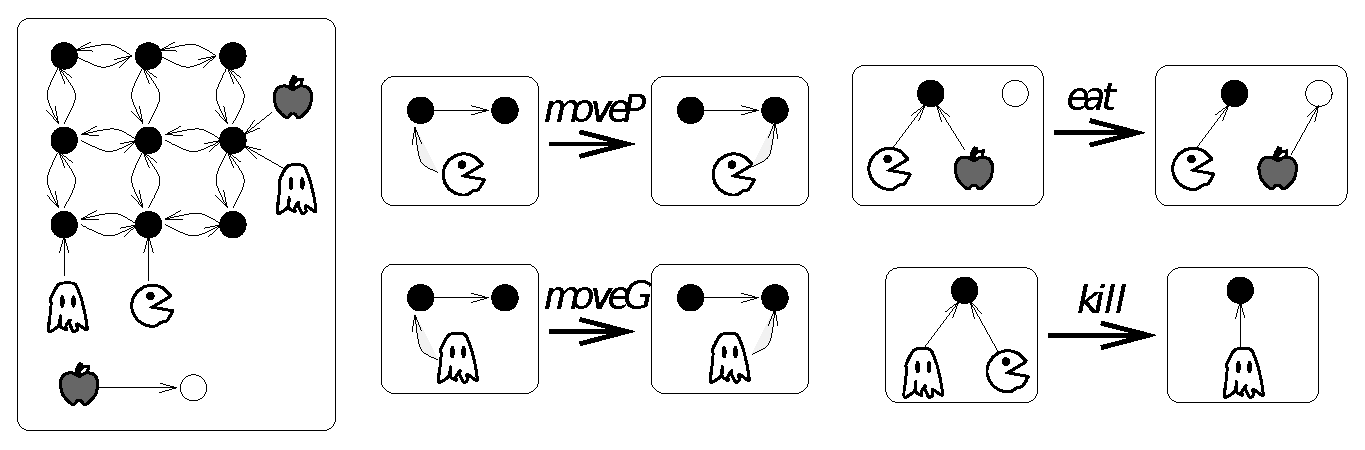
\includegraphics[height=3cm, keepaspectratio]{./pacman/gramatica.eps}

\ei 

\end{frame}
%--------------------------------------------------------------------%

%---------------------------------------------------------------------%
\begin{frame}{\textit{Aplicações de Regras em Gramáticas de Grafos}}

\centering
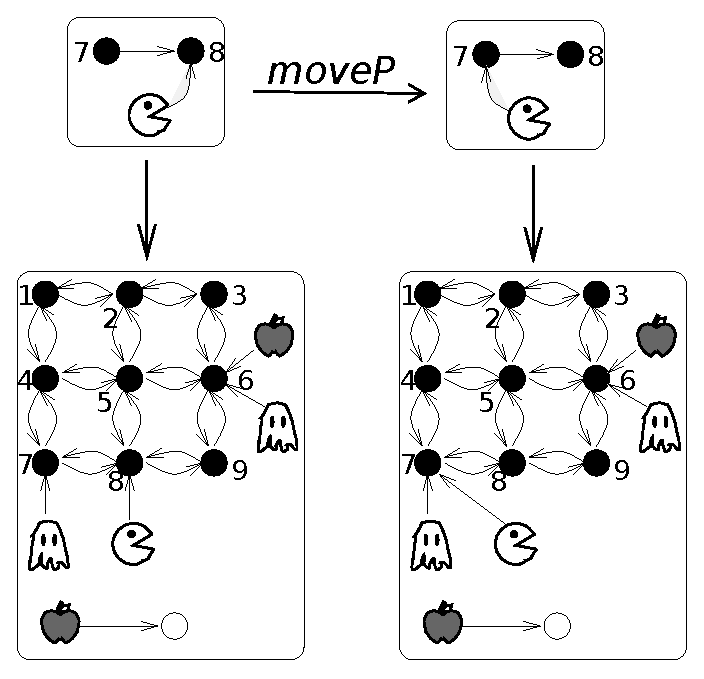
\includegraphics[height=0.8\paperheight,keepaspectratio]{./pacman/ex_aplic_1.eps}

\end{frame}

%---------------------------------------------------------------------%

\begin{frame}{Ferramenta desenvolvida: \emph{Verigraph} I}

\hfill
\bi

    \tm Necessidade de uma Ferramenta Integrada. \\ 

    \vspace{0.25cm}
    \tm Ferramentas Existentes: \\
        \be
            \tm AGG;
            \tm Groove;
            \tm Henshin;
            \tm Outras...
        \ee

    \vspace{0.25cm}
    \tm Funcionalidades Implementadas: \\
        \be
            \tm \textcolor{red}{Análise de Conflitos};
            \tm \textcolor{red}{Análise de Dependências};
            \tm Regras Concorrentes;
            \tm \textcolor{red}{Conflitos Interníveis (1ª e 2ª Ordem)}.
            \tm \textcolor{red}{Model-Checker em Lógica CTL}.
        \ee
    \ei

\end{frame}

%---------------------------------------------------------------------%

\begin{frame}{Análise de Par Crítico}

\bi
    \tm O que é Análise de Par Crítico? \\
        \vspace{0.15cm}
        \begin{figure}
            \centering 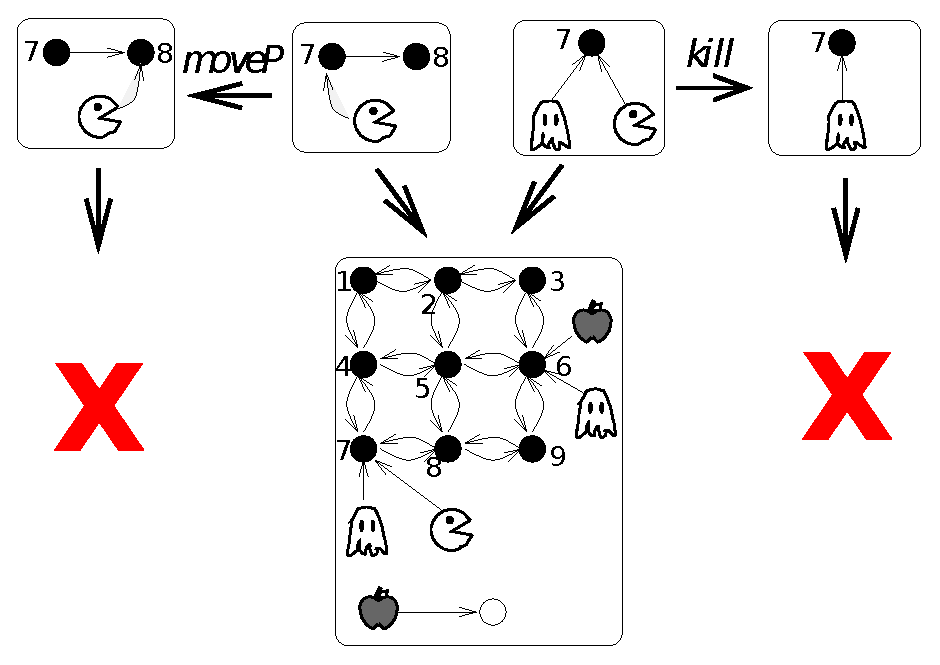
\includegraphics[height=3cm, keepaspectratio]{./pacman/ex_conflito.eps}
            \caption{Exemplo de conflito detectado pela Análise de Par Crítico}
        \end{figure}
        
    \vspace{0.5cm}
    \tm Qual a vantagem da Análise de Par Crítico?
    
\ei 

\end{frame}    

\begin{frame}{Análise de Par Crítico - Exemplo}

\bi
    \tm Tabelas: \\
        \vspace{0.5cm}
        \begin{minipage}{0.45\linewidth}
        \begin{table}
            \newcolumntype{g}{>{\columncolor{gray}}l}
            \newcommand{\green}{\cellcolor{green!25}}
            \newcommand{\red}{\cellcolor{red!25}}
            
            \centering \small
            
            \begin{tabular}{|g|c|c|c|c|}
            \hline \rowcolor{gray}
            & 1   & 2       & 3       & 4       \\ \hline
            1 moveP & \red 3   & \green 0 & \red 1   & \red 1   \\ \hline
            2 moveG & \green 0 & \red 3   & \green 0 & \red 1   \\ \hline
            3 eat   & \green 0 & \green 0 & \red 6   & \green 0 \\ \hline
            4 kill  & \red 1   & \green 0 & \red 1   & \red 3   \\ \hline
            \end{tabular}
            
            \caption{Análise de Conflitos}%
            
        \end{table}
        \end{minipage}
        \hspace{0.5cm}
        \begin{minipage}{0.45\linewidth}
        \begin{table}
            \newcolumntype{g}{>{\columncolor{gray}}l}
            \newcommand{\green}{\cellcolor{green!25}}
            \newcommand{\blue}{\cellcolor{blue!25}}
            
            \centering \small
            
            \begin{tabular}{|g|c|c|c|c|}
            \hline \rowcolor{gray}
                    & 1        & 2        & 3        & 4        \\ \hline
            1 moveP & \blue 4  & \green 0 & \blue 1  & \blue 2  \\ \hline
            2 moveG & \green 0 & \blue 4  & \green 0 & \blue 1  \\ \hline
            3 eat   & \blue 1  & \green 0 & \green 0 & \blue 1  \\ \hline
            4 kill  & \green 0 & \blue 1  & \green 0 & \green 0 \\ \hline
            \end{tabular}
            
            \caption{Análise de Dependências}%
            
        \end{table}
        \end{minipage}
        
    \tm Grafo: \\
        \begin{figure}
            \centering 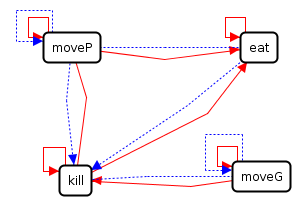
\includegraphics[height=3cm, keepaspectratio]{./pacman/grafo_cpa.png}
            \caption{Grafo de Conflitos de Dependências}
        \end{figure}
\ei

\end{frame}
%---------------------------------------------------------------------%

\section{Desenvolvimento}

\begin{frame}{Contribuições}

\bi
   \tm Implementação da busca de \emph{matches}:
        \bi
            \tm Amplamente utilizado para análises em \emph{GG};
            \tm Algoritmo de busca exaustiva - \emph{Isomorfismo de Grafos};
            \tm Melhorias de Eficiência.
        \ei 
        
    \vspace{0.25cm}
    \tm Contribuição na implementação da Análise de Par Crítico;
    
    \vspace{0.25cm}    
    \tm Medidas de desempenho da ferramenta.
    
\ei
\end{frame}

\begin{frame}{Comparação de Desempenho}
    
    \begin{table}[]
        \newcolumntype{g}{>{\columncolor{gray}}l}
        \centering \small
    
        \begin{tabular}{|g|c|c|}
             \hline \rowcolor{gray}
                          & AGG     & Verigraph \\ \hline
             Conflitos    & 0,964 s & 0,14 s    \\ \hline
             Dependências & 0,658 s & 0,21 s    \\ \hline
        \end{tabular}
        \caption{Comparação de desempenho entre ferramentas - Gramática Exemplo}
    \end{table}
    
    \begin{table}[]
        \newcolumntype{g}{>{\columncolor{gray}}l}
        \centering \small
    
        \begin{tabular}{|g|c|c|}
             \hline \rowcolor{gray}
                          & AGG      & Verigraph \\ \hline
             Conflitos    & 15,146 s & 1,62 s    \\ \hline
             Dependências & 17,818 s & 3,50 s    \\ \hline
        \end{tabular}
        \caption{Comparação de desempenho - Gramática com 16 Regras (Gramatica \emph{Mutex} presente no repositório do \emph{Verigraph\cite{verigraph}}}
    \end{table}
    
\end{frame}

\section{Conclusão}

\begin{frame}{\textit{Verigraph} - Considerações Finais}

\bi
    \tm Ferramenta Integrada de Análises utilizando GG;

    \vspace{0.25cm}
    \tm Desempenho comparável à ferramentas existentes;

    \vspace{0.25cm}
    \tm Grande Extensibilidade;
    
    \vspace{0.25cm}
    \tm Código fonte muito próximo à teoria;
    
    \vspace{0.25cm}
    \tm Licença de Código Aberto.
\ei

\end{frame}


\begin{frame}{\textit{Verigraph} - Futuro}

\bi
    \tm Funcionalidades Futuras: \\
        \be
            \tm \textcolor{red}{Geração Automática de Testes};
            \tm Novos modelos de Transformação de Grafos;
            \tm Evolução de Gramáticas de Grafos;
            \tm Grafos com Atributos;
            \tm \textit{Graph Constraints};
            \tm Interface Gráfica;
            
        \ee
\ei
\end{frame}



%----------------------------------------------------------------------------------%
\begin{frame}{References}
\nocite{*}
    \begingroup
        \renewcommand{\section}[2]{}
            \bibliographystyle{plain}
            \bibliography{apresentacao.bib}
    \endgroup
\end{frame}
%----------------------------------------------------------------------------------%

\begin{frame}{Agradecimentos}

\centering


\includegraphics[width=5cm, keepaspectratio]{./Imagens/logo-propesq.png} \\
\vspace{1cm}
\includegraphics[width=5cm, keepaspectratio]{./Imagens/logo_cnpq.eps}


\end{frame}

\titlepageINF


\end{document}
